\centering
\begin{subfigure}[t]{0.48\textwidth}
  \centering
  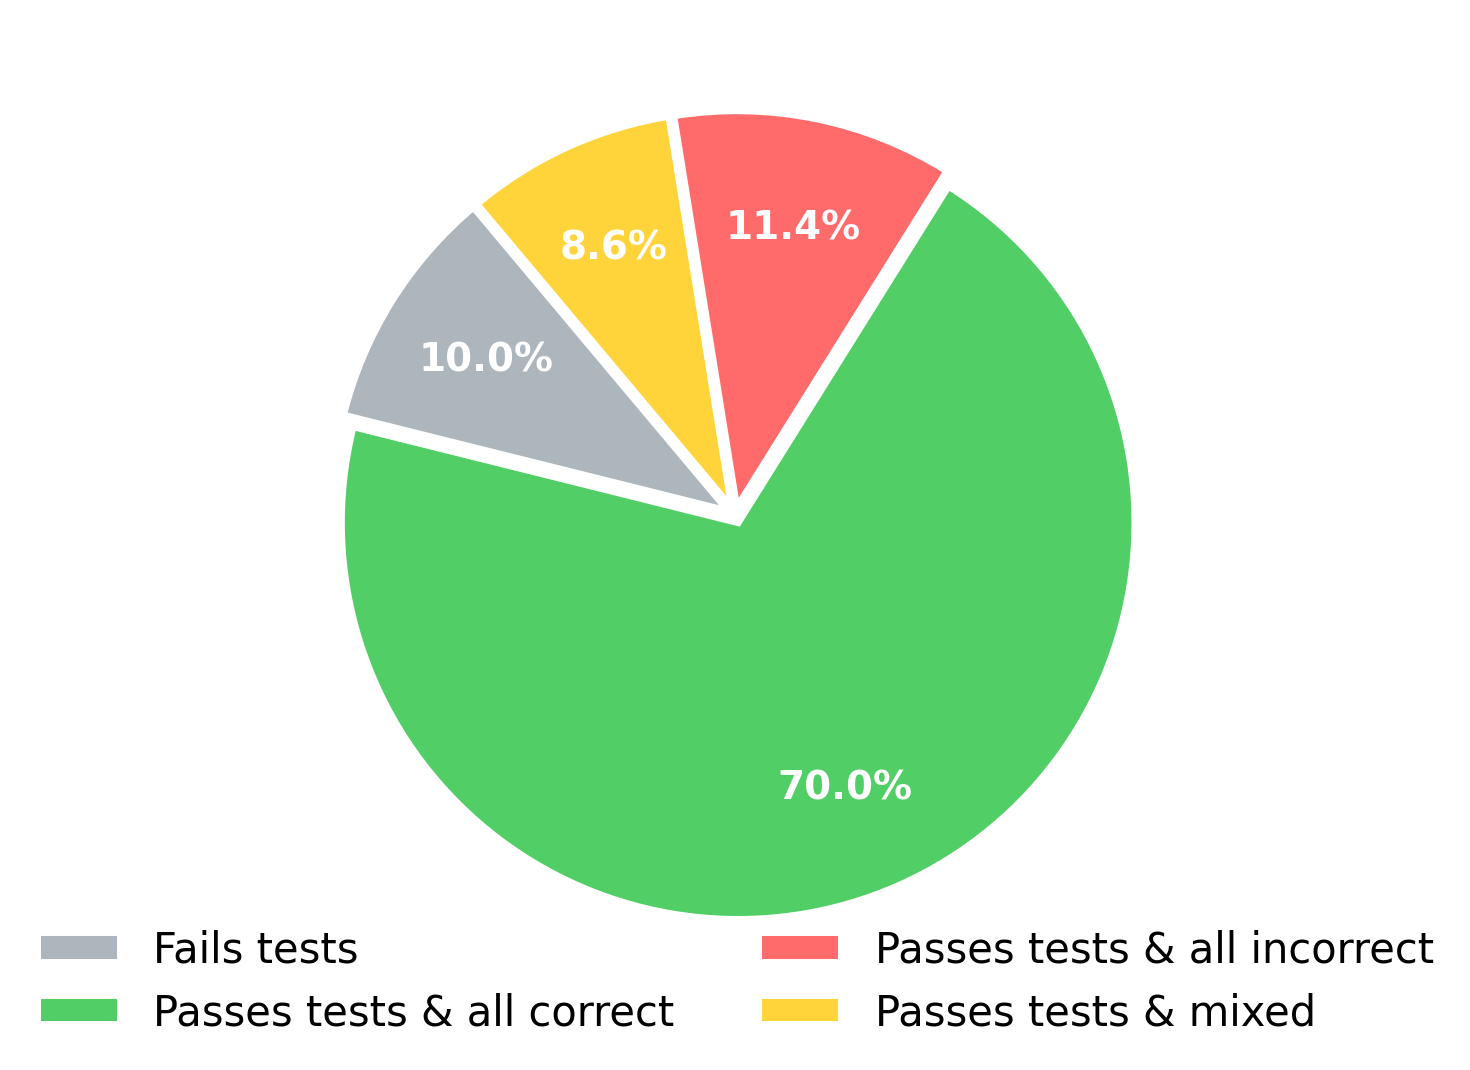
\includegraphics[width=\linewidth]{figures/branch_a2_pass_at_k.png}
  \caption{Unit-test reward (Branch A). Of 70 problems, $70.0\%$ pass the generated tests and are also judged correct against the gold-standard Verus specification. The remaining $20.0\%$ pass the tests despite being incorrect ($11.4\%$ all incorrect, $8.6\%$ a mix of correct and incorrect across the $5$ samples) -- these are reward hacks. The final $10.0\%$ fail the tests outright.}
  \label{fig:results:branch-a}
\end{subfigure}
\hfill
\begin{subfigure}[t]{0.48\textwidth}
  \centering
  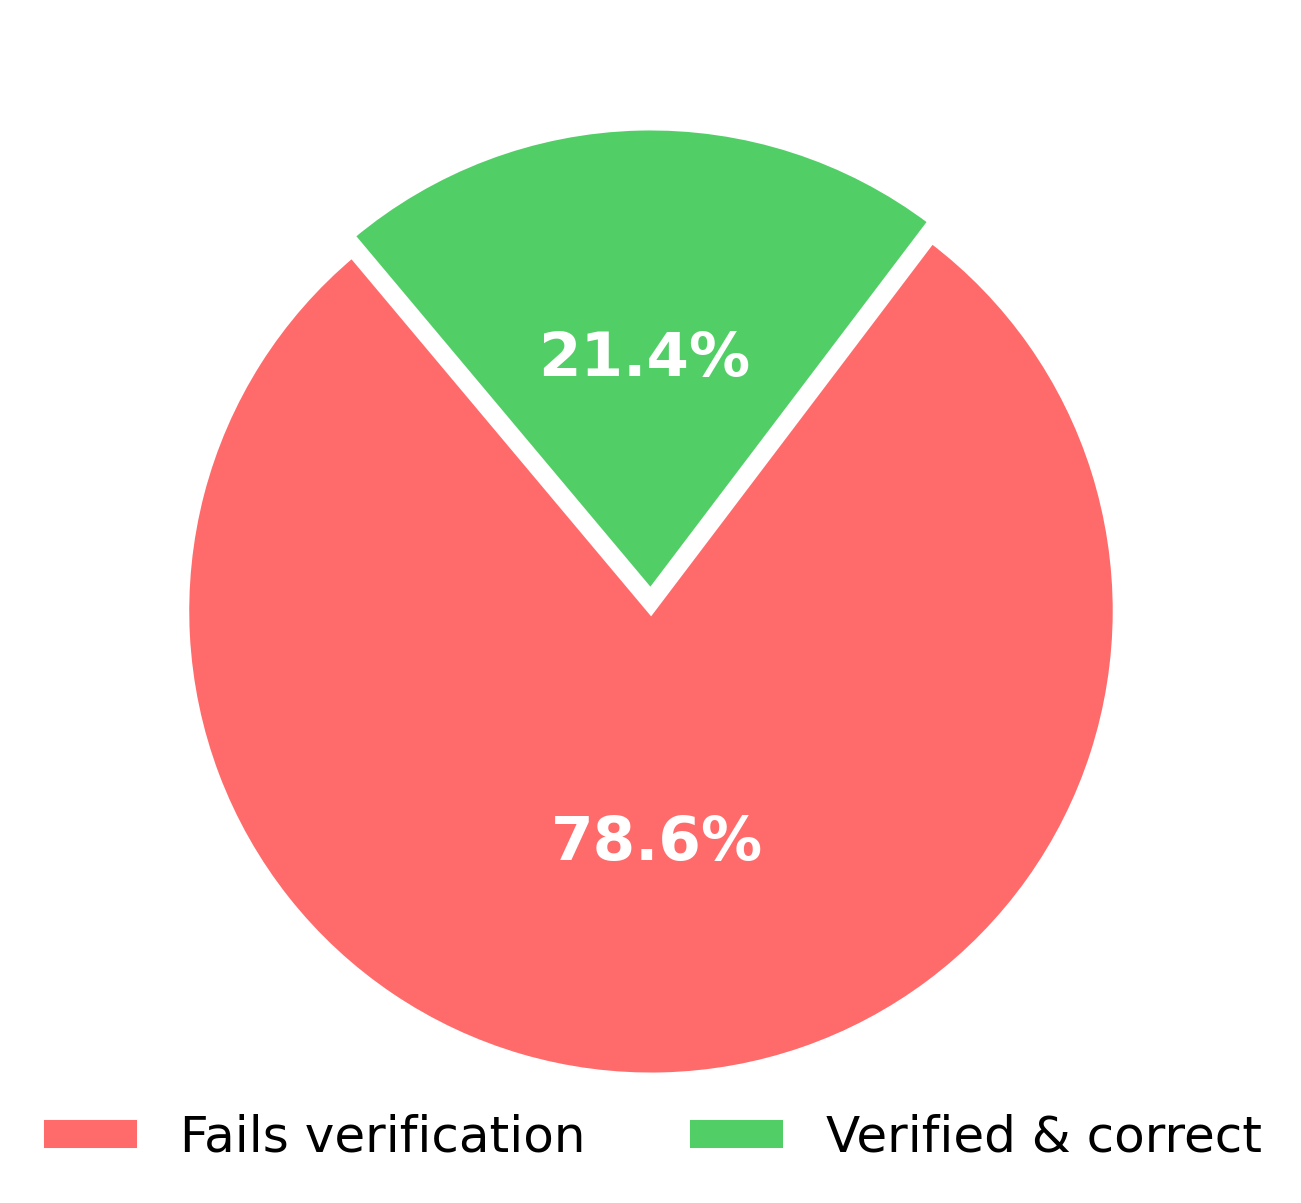
\includegraphics[width=\linewidth]{figures/branch_b_pass_at_k.png}
  \caption{Formal-spec reward (Branch B). Of 70 problems, $21.4\%$ are verified by Verus against the generated specification and judged correct against the gold-standard. The remaining $78.6\%$ fail verification. Crucially, $0\%$ of samples passed verification while being incorrect: with formal specifications, the model never reward-hacked.}
  \label{fig:results:branch-b}
\end{subfigure}
\caption{Outcome breakdown across $70$ HumanEval-Verus problems with Qwen3-Coder at pass@$5$. Reward hacking (passes the in-loop reward signal but is incorrect under the gold-standard spec) accounts for $20\%$ of unit-test outcomes (left) but $0\%$ of formal-spec outcomes (right).}
\label{fig:results-pass-at-k}
